\documentclass{book}

\usepackage{listings}
\usepackage{xcolor}
\usepackage{colortbl}
\usepackage{hyperref}
\hypersetup{
    colorlinks=true,
    linkcolor=blue,
    citecolor=blue,
    urlcolor=blue
}
\usepackage{marginnote}


% vim:set errorformat="":
\usepackage{amsmath}
\usepackage{amsfonts}
\usepackage{amssymb}
\usepackage{xcolor}
\usepackage{colortbl}
\usepackage{marginnote}
\usepackage{wrapfig}
\usepackage{graphicx}
\usepackage{lipsum}
\usepackage{array}
\usepackage{tabularx}
\usepackage{environ}
\usepackage{bussproofs}
\usepackage{exercise}
\usepackage{imakeidx}
\usepackage[normalem]{ulem}
%\usepackage{fontspec} % xelatex only
\usepackage{hyperref} % must be the last one
\hypersetup{
    colorlinks=true,
    linkcolor=blue,
    citecolor=blue,
    urlcolor=blue
}
\renewcommand{\ExerciseHeader}{\medskip\noindent\textbf{\ExerciseName~\ExerciseHeaderNB.~\ExerciseHeaderDifficulty}\emph{\ExerciseHeaderTitle}\\~\\}
\renewcommand{\AnswerHeader}{\medskip\noindent{\textbf{Answer of \ExerciseName~\ExerciseHeaderNB}\\}}

\usepackage[skins,listings]{tcolorbox}
\usepackage{boolexpr,ifthen}
\definecolor{dkblue}{rgb}{0,0.1,0.5}
\definecolor{lightblue}{rgb}{0,0.5,0.5}
\definecolor{dkgreen}{rgb}{0,0.4,0}
\definecolor{dk2green}{rgb}{0.4,0,0}
\definecolor{dkviolet}{rgb}{0.6,0,0.8}
\definecolor{mantra}{rgb}{0.2,0.6,0.2}
\definecolor{gotcha}{rgb}{0.8,0.2,0}

\def\lstlanguagefiles{defManSSR.tex}
\lstset{language=SSR}
\newcommand{\mcbimpl}[1]{\lstinline/?$_{#1}$/}
\newcommand{\mcbimplm}[1]{\mbox{?}_{#1}}

\newcommand{\lib}[1]{\textsf{#1}}

\newcommand{\C}[1]{\mbox{\lstinline`#1`}}
\newcommand{\D}[1]{\mbox{\lstinline'#1'}}
\let\L=\lstinline

% Highlights identifiers, |* id *| in underlined red, can we do better?
\lstset{moredelim=[is][\color{red}\bfseries\ttfamily\underbar]{|*}{*|}}
\lstset{moredelim=[is][\ttfamily\uwave]{|==}{==|}}
\lstset{moredelim=[is][\ttfamily\underbar]{|--}{--|}}

\newcommand\Chapter[2]{\chapter
  [#1\hfil\hbox{}\protect\linebreak{\itshape#2}]
  {#1\\ [2ex] {\Large \itshape #2}}
  \markboth{\MakeUppercase{\chaptername\ \thechapter.\ #1}}{}}

\newcolumntype{V}{>{\centering\arraybackslash} m{0\linewidth} }

\newcommand{\gotcha}[1]{
\begin{center}
\begin{tcolorbox}[colframe=gotcha,
	center title,
	title={\textcolor{white}{\textsf{\Large\textbf{Warning}}}}]
\begin{tabular}{lV}
\begin{minipage}{0.86\textwidth}
\vspace{1em}
#1
\end{minipage}
&
\warnsign{1cm}
\end{tabular}
\end{tcolorbox}
\end{center}}

\newcommand{\mantra}[1]{
\begin{center}
\begin{tcolorbox}[colframe=mantra,
	center title,
	title={\textcolor{white}{\textsf{\Large\textbf{Advice}}}}]
\begin{tabular}{lV}
\begin{minipage}{0.86\textwidth}
\vspace{1em}
#1
\end{minipage}
&
\coqhead{1cm}
\end{tabular}
\end{tcolorbox}
\end{center}}

\newcommand{\coqhead}[1]{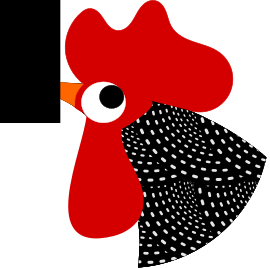
\includegraphics[width=#1]{../artwork/smallpantade}}
\newcommand{\warnsign}[1]{\includegraphics[width=#1]{../artwork/Ambox_warning_pn}}

\newcommand{\mcbpplevel}[1]{
\switch[#1=]
\case{1}
\case{2} \hspace{0.6cm} \coqhead{0.6cm}
\case{3} \coqhead{0.6cm} \coqhead{0.6cm}
\otherwise Please use \textbackslash mcbLEVEL
\endswitch
}
\newcommand{\mcbpptxtlevel}[1]{
\switch[#1=]
\case{1}
\case{2} $(\star)$
\case{3} $(\star\star)$
\otherwise Please use \textbackslash mcbLEVEL
\endswitch
}


\newcommand{\mcbvarreset}{
\mcbLEARN{Please use \textbackslash mcbLEARN}
\mcbREQUIRE{Please use \textbackslash mcbREQUIRE}
\mcbPROVIDE{Please use \textbackslash mcbPROVIDE}
\mcbNOTES{}
\mcbLEVEL{4}}

\newcommand{\mcbLEARN}[1]{\def\mcbvarLEARN{#1}}
\newcommand{\mcbREQUIRE}[1]{\def\mcbvarREQUIRE{#1}}
\newcommand{\mcbPROVIDE}[1]{\def\mcbvarPROVIDE{#1}}
\newcounter{mcbvarLEVEL}
\newcommand{\mcbLEVEL}[1]{\setcounter{mcbvarLEVEL}{#1}}
\newcommand{\mcbNOTES}[1]{\def\mcbvarNOTES{#1}}
\newcounter{mcbvarTMP}

\newcommand{\mcbsection}[1]{
\setcounter{mcbvarTMP}{1}
\ifthenelse{\equal{}{\mcbvarNOTES}}{\setcounter{mcbvarTMP}{0}}{}
\section[#1 \mcbpptxtlevel{\value{mcbvarLEVEL}}]{#1}
\smash{\raisebox{0.7cm}{\hspace{0.92\textwidth}\mcbpptxtlevel{\value{mcbvarLEVEL}}}}
%\marginnote{\small\begin{tabular}{p{3.8cm}}\hline
%\textbf{Learns} \mcbvarLEARN \\
%\textbf{Requires} \mcbvarREQUIRE \\
%\textbf{Provides} \mcbvarPROVIDE \\
%\textbf{Level} \arabic{mcbvarLEVEL} \\
%\switch[\value{mcbvarTMP}=]
%\case{0}
%\case{1} \textbf{Note} \mcbvarNOTES \\
%\endswitch
%\hline
%\end{tabular}\\~\\
%}
\mcbvarreset{}
}

\newcommand{\mcbsubsection}[1]{
\setcounter{mcbvarTMP}{1}
\ifthenelse{\equal{}{\mcbvarNOTES}}{\setcounter{mcbvarTMP}{0}}{}
\subsection[#1 \mcbpptxtlevel{\value{mcbvarLEVEL}}]{#1}
\smash{\raisebox{0.7cm}{\hspace{0.92\textwidth}\mcbpptxtlevel{\value{mcbvarLEVEL}}}}
%\marginnote{\small\begin{tabular}{p{3.8cm}}\hline
%\textbf{Learns} \mcbvarLEARN \\
%\textbf{Requires} \mcbvarREQUIRE \\
%\textbf{Provides} \mcbvarPROVIDE \\
%\textbf{Level} \arabic{mcbvarLEVEL} \\
%\switch[\value{mcbvarTMP}=]
%\case{0}
%\case{1} \textbf{Note} \mcbvarNOTES \\
%\endswitch
%\hline
%\end{tabular}\\~\\
%}
\mcbvarreset{}
}


\newcommand{\mcbsubsubsection}[1]{
\setcounter{mcbvarTMP}{1}
\ifthenelse{\equal{}{\mcbvarNOTES}}{\setcounter{mcbvarTMP}{0}}{}
\subsubsection[#1 \mcbpptxtlevel{\value{mcbvarLEVEL}}]{#1}
\smash{\raisebox{0.7cm}{\hspace{0.92\textwidth}\mcbpptxtlevel{\value{mcbvarLEVEL}}}}
%\marginnote{\small\begin{tabular}{p{3.8cm}}\hline
%\textbf{Learns} \mcbvarLEARN \\
%\textbf{Requires} \mcbvarREQUIRE \\
%\textbf{Provides} \mcbvarPROVIDE \\
%\textbf{Level} \arabic{mcbvarLEVEL} \\
%\switch[\value{mcbvarTMP}=]
%\case{0}
%\case{1} \textbf{Note} \mcbvarNOTES \\
%\endswitch
%\hline
%\end{tabular}\\~\\
%}
\mcbvarreset{}
}
\mcbvarreset{}

\newbox{\devnull}
\NewEnviron{coqdef}[1]{}

\newcommand{\coqrun}[2]{}

\newtcblisting[auto counter]{coq}[2]{
	listing engine=listings,
	listing options={numbers=left,numberstyle=\tiny,
	                 aboveskip=0mm,belowskip=0mm,
		         xrightmargin=0mm,xleftmargin=0mm},
	%on line,
	before={\noindent},
	after={\hfill},
	listing only,
	fonttitle=\small\sffamily,%\bfseries,
	boxrule=0.2mm,top=1mm,bottom=1mm,
	#2
}
\newtcblisting{coqout}[2]{
	listing engine=listings,
	listing options={aboveskip=0mm,belowskip=0mm,
	                 xrightmargin=0mm,xleftmargin=0mm},
	%on line,
	before={\noindent},
	after={\hfill},
	listing only,
	fonttitle=\small\sffamily,%\bfseries,
	boxrule=0.2mm,top=1mm,bottom=1mm,
	#2
}


\title{The Book}
\author{Assia, Enrico, \ldots (you are welcome)}

\begin{document}
\maketitle
\tableofcontents{}

\setcounter{chapter}{-1}
\chapter{The essence of math comp}

\section{challenges faced and tools adopted}
(tools in a broad sense, the logic is a tool, coq is a tool, the plugin
is a tool, the ssr style is a tool,...)

Challenges:
\begin{itemize}
\item large body (scale up), make proofs small and robust.
	We need to say that we do use "deterministic automation".
	Use Laurent's data on de bruijn factor.
\item model the use of math notations, their role in proofs, model proofs (also
	it is about reasoning, not just computations). Another way to say that
	is: model Bourbaki (rationalization of Math via structure/interfaces)
	but not the first book (set theory) that is replaced by CIC (link with
	section computational thinking).
\end{itemize}

We build on Coq and an extension.  The main tools follow (in random order):

\section{Computational Thinking}\label{ch:compthink}

This section should motive the activity of formalizing mathematics
with the {\bf Coq} proof assistant, emphasizing its computing skills,
and as opposed to other foundations like HOL. However the challenge is
to keep mathematicians as the privileged target, while motivating the
ssr approach to a CS oriented reader.

See \verb+../coq/ch0.v+.

Aim of the chapter:
\begin{itemize}
\item should sound natural and easy to a CS person (but with the ssr twist)
\item should sound different but well motivated to a Coq user (do show, maybe in
  the exercises, that leqn is 100 times better than "Inductive le").  Try to
  reproduce the shock we had the first time we used Boolean predicates.  It may
  help to compare, in the *advanced* section, the approach with the standard
  one, so that one sees two proof scripts in the same page.
\end{itemize}

\section{logic programming ... type inference}
to model proof search, give a meaning to notations, teach coq the
work an informed reader does (contextualizing otherwise ambiguous
notations, knowledge of interface/instance of algebraic structures).

relation with proof search: no "blind" proof search (easy, ad-hoc, pervasive
v.s. advanced, generalistic, potentially expensive and unstable).

\section{automation in tactics}
the main points:
\begin{itemize}
\item 1/3 is rewrite, term selection/search (one does not need to reach a sub
	formula as a goal in order to make progress for example, no monkey
	puzzle as in GG terminology).
\item Create a formula without writing it: some advanced forms of forward
	reasoning tactics to deal with symmetries, generalizations (boils down
	to syntesize the cut formula out of the minimum possible user input, as
	in a text where one says "similarly to that, we can also prove that".
	(this is not very pervasive, dunno if it is worth putting it here in
	this chapter).  Also elim does that. (technically also rewrite, but we
	may want to separate things)
\end{itemize}
This section is were one talks about the plugin, and some of the main design
points of tactics: compositional (a language, not a list of commands),
predictable (documented!!!), finally compact (symbols for uninteresting steps).

\section{discipline}
MAKE an howto out of that.
Maybe one should also add a few notes on the style in scripts? like:
\begin{itemize}
\item you must be able to model (at least) 1 proof step in a sentence (line),
  e.g. "rewrite preparegoal dostep ?cleanup."
\item uninteresting/recurrent lemmas/steps should be small (short names, easy to
  gray out)
\item lemma statements are designed, not just written, having in mind their use
      (forward, backward, implicit argumets, arguments order)
      and the class of trivial hypotheses since an extra hyp that is proable
      triviality (via //, hint resolve, cnaonical) is for free. E.g.
      "x \\is a toto", "0 <= n", ...
\item also not every possible lemma, but a few that combine well
\item proofs/definitions are reworked many times, why (understand recurrent
  proof schemas, compact, factor, make more stable/robust) and what is needed
  (like meaningful names, clear structure)
\end{itemize}

\section{trivial=implicit (for a trained mathematician)}
The idea is to try to identify what is trivial (mathematically speaking)
and be sure you can model it as such:
\begin{itemize}
\item (level basic) make explicit the trivialities of each theory (what one
	expects to be proved by //). 
\item (level advanced) when you do new stuff, you must decide what is
	trivial/implicitly proved.
\item (hard) which technique to make Coq prove it automatically (hint resolve,
	canon, comput... in the type)
\end{itemize}

This may also be another way present the whole chapter

\mantra{(basic) if you see toto=false you should perform the case analysys via fooP}


\part{The art of formalizing}

\chapter{Logics}

From calculability to proofs, hence the CC, and the fact that
reasoning principles without a computational content become axioms.

This is a non technical chapter and message should be:
\begin{itemize}
\item instantiation of a universal statement is application (also the pair)
\item Excluded middle is not available by default (choice?)
\item Conversion as a pervasive indistinguishably, what inside
  (beta, definition unfolding,...)
\item Dependent types: eq, sigma (which example?)
\end{itemize}

One options is: avoid relating type theory and other logics. We say:
we have a formal game where the basic elements are programs/functions
that come with types to avoid confusion. full stop. (no relation with
proof theory, set theory). maybe mention that roots are in calculability (hence
the choice to pick functions as primitive and not sets). This is lucky because
(computable) functions are today executable by a computer.  Still not all
concepts are "computable" hence some principles are problematic: EM,.... we
mainly stay in the lucky fragment (again no propaganda on intuitionistic logic,
constructive math; just a mention).

\chapter{Programming}

Presentation of inductive data structures, recursive programs on these
data.
Bool, Boolean connectives, Boolean reflection (cf
ch. \ref{ch:compthink}), views.
Examples of equality tests ($==$, with a forward reference to
explain the magic if needed), operations on sequences, nats,
exercises on prime, div.

\chapter{Proofs}

Where one learns to do proofs.
Boolean reflection in practice, views, discussion on the definition of leq,
proofs on things defined in the
previous chapter, associated tactics, exercises on prime, div,
binomial, etc.

spec? A new vernacular to declare specs without typing coinductive and
by writing explicitly the equations.

\chapter{Type inference/Genericity}

put here a minimalistic presentation of records.

Implicit arguments (Is it possible to survive without implicit
argument up to this point? We should probably use them plus forward
references to here), canonical structures. Combining with
notations. Now the real $==$. 

\chapter{Mixing data and proofs}
Boolean sigma types, records, coercions, UIP. Examples: ordinals,
tuples (not their use which requires CS). This chapter might come
after some presentation of basic canonical structures, i.e. reorganize
the content between this chapter and the next.

example of tuples here? better ordinals?

GG: makes many points here (not fully understood by Enrico):
\begin{itemize}
\item ordinals/tuples are easy to use but hard to build
\item it is a tradeoff, but is not clear if we can give hints on when
	a specific datatype like ordinals is better that unpackaged
	stuff.
\end{itemize}

UIP is advanced, the basic user should just be told that putting
bools inside a record is just fine.

\begin{itemize}
	\item record (flat)
	
\end{itemize}


\chapter{Hierarchy}
Packaging records, the bigop hierarchy.
Scaling with packed classes and mixins, to the ssralg
hierarchy. Presentation of the content of ssralg in terms of structures
and of the theory? Should the latter be a separate chapter.

Maybe a plugin for a new vernacular to script the creation/declaration
of structures/instances so that the level basic can touch the argument
easily.

Explain what the abstraction barrier is (like unfolding a GRing projection)

\gotcha{if you see GRing.toto then you broke an abstraction barrier}

\mantra{
	if you have a proof in mind, don't let the system drive you
        to another, less clean and abstract, proof.
}

Declaring an instance is hard... we need to document the multuiple processes 
for each structure in each hierarchy and possibily make a program out of it.

\chapter{Larger scale reflection (out of place)}
Four colours, decomposition in primes, example in peterfalvi. In
particular example where a case analysis does not follow the
constructors of an existing inductive type: then craft an ad hoc one
to hint the proof. This topic is probably at a wrong place.

\part{Mathematics in Mathematical Components}

\section{STYLE of these chapters}
These chapters hopefully in the following style:
\begin{itemize}
\item first math mode to review the (not so standard) definitions and
\item then touch some real proof script to show why/how the definition
  make it possible to model the proofs (as they are in math)
\item use the (few) examples to illustrate a cool proof strategy if
  any (not necessarily typical of the math subject, but that happens to
  be there, like in OOTHM paper: circular leq, symmetries, ad hoc
  decision procedure, ...)
\item try hard to show how CIC helps (which feature: HO, computation, dependent
	types \ldots), so that at the end we can sum up and make a synthesis of
	all that.
\end{itemize}

Maybe it is simpler to do it in 2 steps:
1) in this second part one identifies where CIC or the SSR style plays a
   crucial role
2) then we advertise these use cases in the first part to motivate
   the techniques, the complexity of the logic...

\chapter{Numbers}

What are the numbers available in the library? How to use them, casts
between types... Non trivial point in the formalisation:
axiomatization, order is defined from norm, partial orders (in
particular for complex numbers).


\chapter{Polynomials, Linear algebra}

2-stage presentation: interface plus explicit. Expansion of
Georges'ITP paper. Here is one of the main application of the choice
operator (complement a base).

\chapter{Quotients}

\chapter{Finite group theory}

Data-structures, how to craft the set of variants of a same theorem to
make the formalization handy. Permutations. Presentations?

\chapter{Representation theory, Character theory}

As an example of application, in particular of the linear algebra
theory.

\chapter{Galois Theory}


\chapter{Real closed fields}

\chapter{Algebraic closure}

\part{Conclusion and perspectives}

Let's be brave:
This part looks back to the techniques, methodologies and achieved
formalized libraries described in the book and summarizes the role
played by each on them, in the spirit of the introduction to the ssr manual.
May be also discusses the possible extensions
(like CoqEAL) or adaptation to the future evolutions of the system and
formalism (Cubical Coq, HITs...).

\part{Annexes}

\chapter{What is done where?}

\chapter{How tos}
suggestions:
\begin{itemize}
\item Get more information when you do not understand the error
  message
\item Search in the library
\item Canonical structures: define a new instance
\item Canonical structures: add a new structure
\item Give a relevant name to the lemma I just stated
\item Forbid unwanted expansions
\item Choose a notation (what not to do...)
\item Compute ``for real'' (Natbin, Coqeal)
\item MathComp script style
\end{itemize}
\chapter{Naming conventions}

\chapter{Index of notations}

\end{document}
